This program is almost fully automatable with macros. Macros
canb e used to perform data analysis as quickly as possible. 
The program is capable of recording macros and running macros. 
The macro file format is simple enough that it is easy write 
or modify macro files by hand.

\begin{SCfigure}[1][hbtp]
    \centering
    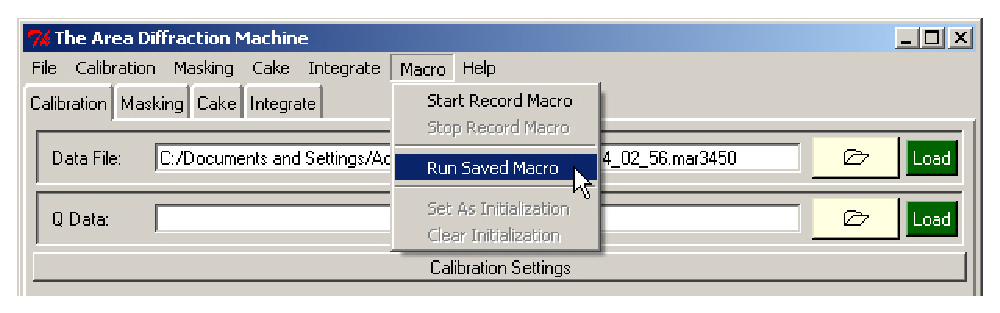
\includegraphics[scale=.75]{figures/macro.eps}
    \caption{The \gui{Macro} menu bar. This is
    where macros are recorded and run.}
    \label{macro_figure}
\end{SCfigure}

\section{Record Macros}

The easiest way to create a macro is to record it. A macro
can be recorded by selecting the \gui{Start Record Macro} 
option in the \gui{Macro} menu 
bar. Figure~\ref{macro_figure} shows the \gui{Macro} menu bar.
After all of the steps that should be recoreded are finished, 
pushing \gui{Stop Record Macro} will save the macro file to
a selectable file.

\section{Run Macros}

The \gui{Run Saved Macro} option in the \gui{Macro}
menu to run a macro file. The program will run all the 
steps in the macro file and then return control of 
the program. This is how analysis can be done with
macro files.

\section{The Macro File Format}

A macro file contains a list of commands which tell the 
program what to do. Each command in the GUI is on its
own line. The syntax for macro commands is pretty 
straightforward. Macro commands are the 
text corresponding to the part of the GUI that does 
the command. For example, to make the macro get the 
calibration data from the header of the image, the macro 
command is \macroline{Get From Header}. To fit the calibration
data from within a macro, the command is 
\macroline{Do Fit}.

Things get more interesting when the GUI item requires
requires doing more then just pushing a button. For 
example, to deselect the \gui{Draw Q Data?} 
check box, the macro needs to specify that the check box
gets deselect instead of selected.
For these, the macro commands need to be followed by
a second line with the particular. For this example, 
we would write
\begin{lstlisting}[caption={'Draw the $Q$ Lines on the Display'}]
Draw Q Data?
    Select
# Or, to not display them:
Draw Q Data?
    Deselect
\end{lstlisting}
It is the same when numbers should be set. To change
a calibration values, the macro would look like:
\begin{lstlisting}[caption={'Input a Number'}]
xc:
    1752.3
beta:
    5.23
\end{lstlisting}
These are treated just the same. The following
macro command would save the cake as an image:
\begin{lstlisting}[caption={'Save the Caked Image'}]
Save Caked Image
    C:/data/cake_output.jpg
\end{lstlisting}

If you look on the first tab, there are three inputs
at the top:
\gui{Get From Header:}, \gui{dark current:}, and 
\gui{Q data:}. The macro command to load any of these
is a little bit ambiguous. When using the actual GUI, 
you would, at least in principle, type in the name of
a file and then press load. But there is no reason to
make the GUI so redundant. So to load in any of these
using a macro command, all you have to do is give the 
name of the input and then the filename. It will 
automatically load the file without you explicitly
giving the \macroline{load} line. So, for example,
to load in the $Q$ data, you would include the 
following lines:
\begin{lstlisting}[caption={'Load the $Q$ Data'}]
Q Data:
    C:/data/q_data.dat
\end{lstlisting}

\section{Looping Over Diffraction Data}
\label{LoopOverDiffractionData}

To analyze a file, the command is just 
\begin{lstlisting}[caption={'Load the Diffraction Data'}]
Data File:
    C:/data/first.mar3450
Get From Header
# ...
\end{lstlisting}
But macros files also allow for an easier way
to loop over many files and perform the same
analysis on all of them.  
To loop over multiple diffraction images at once,
you could simply give more files after the first 
one. The loop will end when 
one of the 3 things in the macro 
file happens: a subsequent line in the macro
file reads \macroline{END LOOP}, more diffraction data
is loaded using the command \macroline{Data File:}, or
the macro file ends. For example, if we look at this 
macro file.
\begin{lstlisting}[caption={'Loop Over Diffraction Data'}]
Data File:
    C:/data/first.mar3450 C:/data/second.mar3450 
Integrate Q Lower?
    .25
Integrate Q-I
END_LOOP
Draw Q Lines?
    Select
# ...
\end{lstlisting}
We see that it would get evaluated just like this
macro file:
\begin{lstlisting}[caption={'An Equivalent Macro'}]
Data File:
    C:/data/first.mar3450 
Integrate Q Lower?
    .25
Integrate Q-I
Data File:
    C:/data/second.mar3450 
Integrate Q Lower?
    .25
Integrate Q-I
Draw Q Lines?
    Select
# ...
\end{lstlisting}
You can even give it whole directories. When
you give it a directory to loop over, the program 
will (non-recursively) look for all the diffraction 
files in that directory and include them in the list. 
For example, if the folder \macroline{C:/data/} contains
only the file \macroline{first.mar3450} and
\macroline{second.mar3450}, an equivalent way of looping
over these files would be to issue the command
\begin{lstlisting}[caption={'Load the Diffraction Data'}]
Data File:
    C:/data/
# ...
\end{lstlisting}
You can put as many folder and files after a 
\macroline{Data File:} line as you wish.
Just make sure to put them all on the same line 
or the program will complain.

\section{The PATHNAME and FILENAME Commands}

Finally, there is a convenience markup which can help
you make fancy macros. Whenever you have loaded data 
in, you can refer to the part name of the current
diffraction file that is loaded using the string
\macroline{PATHNAME} and you can refer to the file
name itself using the string \macroline{FILENAME}. 
So, in our previous example, if we had loaded the
file \macroline{C:/data/second\_file.mar3450},
\macroline{PATHNAME} would get chaned into 
\macroline{C:/data} and \macroline{PATHNAME} would
get evaluated to \macroline{second\_file} without
the extension. In effect, you can imagine building 
back the full name from \macroline{PATHNAME} and
\macroline{FILENAME} using an equation line
\begin{equation*}
    \text{\macrolinenoquotes{C:/data/second\_file.mar3450}=
    \macrolinenoquotes{FILENAME/PATHNAME.mar3450}}
\end{equation*}
These commands are useful because they allow you to
loop over many files at once but still save things 
in useful places and with useful names. It would be
easy, for example, to save the intensity data you
calculate for each file being looped over using the 
macro command:
\begin{lstlisting}[caption={'Using the FILENAME and PATHNAME Markup'}]
Save Integration Data
    FILENAME/PATHNAME\_int.dat
\end{lstlisting}
This would save, for example, 
\macroline{C:/data/first.mar3450}'s intensity data to
\macroline{C:/data/first\_int.dat},
\macroline{C:/data/second.mar3450}'s intensity data 
to \macroline{C:/data/second\_int.dat}, and the
same for all the others. This feature lets you have
the macro to save each of the files to the right place
and give it a useful name.

\section{Loops Over Multiple Images}

We know from chapter~\ref{viewing_data} that
you can load in multiple diffraction images and add them
together. But we have not yet talked about how this can
be done inside of a macro. The syntax is pretty straight
forward. We introduce a new macro command named
\macroline{Multiple Data Files} which signifies that
many files should be loaded. To load in multiple files
and have their intensities added, this command must be 
followed by a list of filenames enclosed within
[ and ] brackets. Keeping with the same example above,
we could load in \macroline{C:/data/first.mar3450} and
\macroline{C:/data/second.mar3450} and have their
intensities added using the command
\begin{lstlisting}[caption={'Add the intensities'}]
Multiple Data Files:
    [C:/data/first.mar3450 C:/data/second.mar3450]
# ...
\end{lstlisting}
The program enforces that
all of the files are in the same folder. This is done
so that that the \macroline{PATHNAME} variable remains 
meaningful when looping over multiple images.

You can then incorporate this into a loop in
one of two ways. First, you can simply put several
of these bracketed lists into the macro and each
of the lists will be analyzed separately. For example,
\begin{lstlisting}[caption={'Loop Over the Analysis'}]
Multiple Data Files:
    [C:/first.mar3450 C:/second.mar3450] [C:/third.mar3450 C:/fourth.mar3450]
# ...
\end{lstlisting}
This will separately loop over \macroline{first.mar3450} 
and \macroline{second.mar3450} added together and then 
\macroline{third.mar3450} and \macroline{fourth.mar3450}
added together. But this gets cumbersome. Alternately,
you can simply take all of the files that you want to be 
added together and analyzed and group them into subfolders. 
Each of the subfolders will contain only files that should
be added together and analyzed. If you then give the
macro the name of the folder containing all these subfolders,
it will loop over all the subfolders. 

For example, suppose we created the folder \macroline{C:/data}.
Inside of this folder is the subfolder \macroline{A}
containing the files \macroline{first.mar3450} and 
\macroline{second.mar3450}. Also inside of the data folder
is the subfolder \macroline{B} containing the files
\macroline{third.mar3450} and \macroline{fourth.mar3450}.
We could do the exact same data analysis as above by 
issuing the macro command with only the data folder name.
\begin{lstlisting}[caption={'Using the Folder Syntax'}]
Multiple Data Files:
    C:/data
# ...
\end{lstlisting}
You can also put as many folders and lists separated
by [ and ] as you wish onto the line and it will loop
over all of them.

Since the macro function insists that all files 
that are added together are in the same folder,
the \macroline{PATHNAME} command will properly expand 
to the path that all of the files that were added 
together have. But since they all have different file 
names, the \macroline{FILENAME} command will always be 
replaced by the string \macroline{MULTIPLE\_FILES}
to avoid ambiguity.

\section{The FOLDERPATH and FOLDERNAME commands}

To facilitate writing macros that load in and 
add together several diffraction images, the program
introduces two new macro commands. The first command is
\macroline{FOLDERNAME} and will always be replaced
by the name of the folder containing the current
diffraction file (or files). Since the macro insists 
that all files are loaded form the same Folder, this
command is unambiguous. Finally, you can use the 
command \macroline{FOLDERPATH}. It will always be 
replaced by the path leading up to the folder 
containing the file. Therefore, we can now specify 
where the current file is by using the macro command
\begin{equation*}
    \text{\macrolinenoquotes{FILENAME/PATHNAME.mar3450}}
\end{equation*}
or the command
\begin{equation*}
    \text{\macrolinenoquotes{FOLDERPATH/FOLDERNAME/FILENAME.mar3450}}
\end{equation*}
Basically, this is useful because if you are adding
together multiple files, you can put them all in a
folder with an interesting name and then name 
the output files something like 
\macroline{FOLDERNAME\_int.dat} so that they are all
given useful names. This is nice because it can, without
loss of generality, be incorporated into a loop. Finally,
the \macroline{FOLDERPATH} command is useful because you
can use it to output files one directory up from where all
the diffraction data is stored.

\section{Setting Colors in a Macro}

There are several places in the program where you can
pick the color of something using a color selector.
It is a little trickier to do.  When you issue a macro 
command that wants to know the color of something, you 
have to tell it what that color is. By far the easiest
way to figure out exactly what the macro line should
loop like is to simply record a macro where select
the color that you want and then copy the macro lines
into your file.

But if you are curious exactly what the format for
colors looks like, you can see that picking a color
will generally look like this:
\begin{lstlisting}[caption={'Use the Folder Syntax'}]
Polygon Mask Color?
    red
\end{lstlisting}
But it is a bit tricky trying to figure out exactly what 
colors will work. Technically, this program will accept 
any color which tk will accept. The colors that tk
will accept by name are all described here:
\url{http://wiki.tcl.tk/16166}. But tk can also accept
colors based upon their RGB value. To specify a color
by its RGB value, the color must be preceded by a \#
and followed by the RGB values in hexadecimal.
Each of the RGB values range from 0 to 255 in
decimal or (00 to ff in hexadecimal).
For example, pure red would be specified by the color
\#ff0000. So we could replace the macro command above
with the identical
\begin{lstlisting}[caption={'Use the Folder Syntax'}]
Polygon Mask Color?
    #ff0000
\end{lstlisting}

\section{Little Tidbits}\label{Little Tidbits}
\begin{itemize}
    \item Any of the macro commands themselves are case
    insensitive. The command \macroline{GeT fRoM hEaDeR} 
    is just as valid as the command 
    \macroline{gET fROM hEADER} and 
    \macroline{Get From Header}. You don't have to sweat it. 
    \item White spaces at the beginning and end of the 
    line are ignored. In the preceding examples, the
    spaces separating macro commands from input values
    such as file names are there only to increase 
    readability. You don't need them if you don't 
    want.
    \item Any new lines in a macro file are ignored.
    \item comment lines of the form 
    \macroline{\# A comment} are ignored.
    \item You don't have to worry about explicitly moving 
    from tab to tab in the computer program. The computer 
    program will move to the right automatically before
    performs the action.
    \item When you issue the macro command \macroline{E:} 
    or \macroline{E Fixed}, the computer program will
    automatically set the GUI to \macroline{Work in eV}.
    If you issue the command or \macroline{lambda:} or
    \macroline{lambda fixed:} then the comptuer program
    will set the GUI to \macroline{Work in Lambda}. You
    can also explicitly set the GUI to either mode using
    the command \macroline{Work in eV} or
    \macroline{Work in Lambda}.
\end{itemize}


\section{Macro Commands}

Below is a table describing all of the macro command 
and exactly what they do.

\begin{center}

\setlongtables % keeps the width uniform across pages
\begin{longtable}{|p{4cm}|p{4cm}|p{7cm}|}
\caption{Macro Commands} \label{grid_mlmmh} \\

\hline \multicolumn{1}{|c|}{Command} & \multicolumn{1}{c|}{Followed By} & \multicolumn{1}{c|}{Effect} \\ \hline 
\endfirsthead

\multicolumn{3}{c}%
{{\bfseries \tablename\ \thetable{} -- continued from previous page}} \\

\hline \multicolumn{1}{|c|}{Command} & \multicolumn{1}{c|}{Followed By} & \multicolumn{1}{c|}{Effect} \\ \hline 
\endhead

\hline \multicolumn{3}{|r|}{{Continued on next page$\ldots$}} \\ \hline
\endfoot

\hline 
\endlastfoot
\multicolumn{3}{|c|}{Program State Macro Commands} \\
\hline 
    \macrolinenoquotes{Work In eV}&None&Change the state of 
        the program so that the energy calibration parameter 
        is inputted in units of electron volts. This is called
        the $eV$ mode of the program. \\
    \macrolinenoquotes{Work in Lambda}&None&Change the state of 
        the program so that the energy calibration parameter
        is inputted instead as a wavelength in units of 
        angstroms. The conversion is done using the formula
        $E=hc/\lambda$. This is called the $\lambda$ mode
        of the program.\\
    \macrolinenoquotes{Work in 2theta}&None&Change the state of
        the program so that caking and intensity integration
        are done of the variable $2\theta$. \\
    \macrolinenoquotes{Work in Q}&None&Change the state of
        the program so that caking and intensity integration
        are done of the variable $Q$. \\
    \hline
    \multicolumn{3}{|c|}{Calibration Values} \\
    \hline
    \macrolinenoquotes{Data File:}&Files \& Directories&Loops 
        over loading in each file.\\
    \macrolinenoquotes{Multiple Data Files"}&
        Files \& Directories&Loops over
        loading several diffraction files and adding
        them together.\\
    \macrolinenoquotes{Dark Current:}&Filename&Loads in the 
        Dark Current.\\
    \macrolinenoquotes{Q Data:}&Filename&Load in the $Q$ data.\\
    \macrolinenoquotes{Standard Q}&q data&Loads in one of the
    standard $Q$ files. This command should be followed by the
    name of the standard Q file as it is displayed by the program
    in the menu bar.\\
    \macrolinenoquotes{Get From Header:}&None&Sets the calibration 
        data to the value stored in the image header.\\
    \macrolinenoquotes{Load From File:}&Filename&Loads a calibration 
        data file.\\
    \macrolinenoquotes{Previous Values}&None&Loads the previously 
        stored calibration values.\\
    \macrolinenoquotes{Save To File}&Filename&Saves the calibration 
        data to a file.\\
    \macrolinenoquotes{xc:}&Number&Sets the $x$ center.\\
    \macrolinenoquotes{xc Fixed:} & \selectordeselect & Sets whether 
        or not to fix the $x$ center while doing the fit.\\
    \macrolinenoquotes{yc:}&Number&Set the $y$ center.\\
    \macrolinenoquotes{yc Fixed:}& \selectordeselect &Sets whether 
        or not to fix the $y$ center while doing the fit.\\
    \macrolinenoquotes{d:}&Number&Set the distance from the 
    sample to the detector.\\
    \macrolinenoquotes{d Fixed:}& \selectordeselect &Sets whether 
        or not to fix the distance while doing the fit.\\
    \macrolinenoquotes{E:}&Number&Sets the energy. If this
        command is run while the program is in $\lambda$ mode,
        the program will switch to $eV$ mode.\\
    \macrolinenoquotes{E Fixed:}& \selectordeselect &Sets whether 
        or not to fix the energy while doing the fit. If this
        command is run while the program is in $\lambda$ mode,
        the program will switch to $eV$ mode.\\
    \macrolinenoquotes{lambda:}&Number&Sets the wavelength. If
        this command is run while the program is in $eV$ mode,
        the program will switch to $\lambda$ mode.\\
    \macrolinenoquotes{lambda Fixed:}& \selectordeselect &Sets 
        whether or not to fix the wavelength while doing the 
        fit. If this command is run while the program is in
        $eV$ mode, the program will switch to $\lambda$ mode.\\
    \macrolinenoquotes{alpha:}&Number&Sets the $\alpha$ angle.\\
    \macrolinenoquotes{alpha Fixed:}& \selectordeselect &Sets whether 
        or not to fix the $\alpha$ angle while doing the fit.\\
    \macrolinenoquotes{beta:}&Number&Sets the $\beta$ angle.\\
    \macrolinenoquotes{beta Fixed:}& \selectordeselect &Sets whether 
        or not to fix the $\beta$ angle while doing the fit.\\
    \macrolinenoquotes{R:}&Number&Sets the rotation angle.\\
    \macrolinenoquotes{R Fixed:}& \selectordeselect &Sets whether 
        or not to fix the rotation angle while doing the fit.\\
    \macrolinenoquotes{pl}&Number&The pixel length of the image.
        This is the width of one pixel (in microns).\\
    \macrolinenoquotes{ph}&Number&The pixel height of the image.
        This is the height of one pixel (in microns).\\
    \macrolinenoquotes{Draw Q Lines?}&\selectordeselect&Sets wether 
        or not to draw constant $Q$ lines on the screen.\\
    \macrolinenoquotes{Draw Q Lines Color?}&color&Sets the color 
        of the constant $Q$ lines that are displayed on 
        top of the diffraction data and the caked data.\\
    \macrolinenoquotes{Draw dQ Lines?}&\selectordeselect&Draw the 
        delta $Q$ lines on the diffraction image.\\
    \macrolinenoquotes{Draw dQ Lines Color?}&color&Change the 
        color of the delta $Q$ lines that are displayed on
        top of the diffraction data and the caked data.\\
    \macrolinenoquotes{Draw Peaks?}&\selectordeselect&
        Display the fit peaks on the diffraction and 
        cake image.\\
    \macrolinenoquotes{Draw Peaks Color?}&color&Change the color of 
        the peaks that are displayed on top of the diffraction
        data and the caked data.\\
    \macrolinenoquotes{Update}&None&Update the diffraction image.\\
    \macrolinenoquotes{Save Calibration}&Filename&Saves the
        current calibration values in the GUI as plaintext
        ASCII to a file.\\
    \macrolinenoquotes{Do Fit}&None&Fit the calibration values to 
        a loaded diffraction image.\\
    \macrolinenoquotes{Make/Save Peak List}&Filename&Creates a peak 
        list just as happens when doing the fit, but instead of 
        acutally doing the fit it saves the peaks as an ASCII file 
        for later use.\\
    \macrolinenoquotes{Use Old Peak List (if possible)?}&
        \selectordeselect&Uses the previously found peak list again 
        when doing the fit.\\
    \macrolinenoquotes{Fit Number of Chi?}&Number&The number of 
        $\chi$ slices around the diffraction image to pick and use 
        when doing the calibration.\\
    \macrolinenoquotes{Stddev}&Number&The $\sigma$ threshold for 
        allowing a peak.\\
    \hline    
    \multicolumn{3}{|c|}{Diffraction Display Options} \\
    \hline
    \macrolinenoquotes{Diffraction Data Colormaps}&A color map name&
        Select the color map to use for the diffraction image.\\
    \macrolinenoquotes{Diffraction Data Invert?}&\selectordeselect&
        Invert the color map that is being used to display
        the diffraction data.\\
    \macrolinenoquotes{Diffraction Data Log Scale?}&\selectordeselect&
        Take the log of all the data points before displaying them.\\
    \macrolinenoquotes{Diffraction Data Low?}&Number from 0 to 1&The 
        normalized intensity value which will be scaled to \%0 of 
        the image brightness when displaying the diffraction image.\\
    \macrolinenoquotes{Diffraction Data Hi?}&Number from 0 to 1&The 
    normalized intensity value which will be scaled to \%100 of the
    image brightness when displaying the diffraction image.\\
    \macrolinenoquotes{Save Diffraction Image}&Filename&Save the 
    diffraction image to a file (possibly including $Q$ lines and 
    peaks.\\
    \hline    
    \multicolumn{3}{|c|}{Masking Macro Commands}\\
    \hline
    \macrolinenoquotes{Do Less Than Mask?}&\selectordeselect&
        Sets whether or not to apply a less than mask to the
        diffraction data.\\
    \macrolinenoquotes{(Pixels Can't Be) Less Than Mask:}&Number&
        Sets the less than mask.\\
    \macrolinenoquotes{Less Than Mask Color?}&color&Sets the
        color that all the less than masked pixels are
        displayed as on the diffraction image and caked image.\\
    \macrolinenoquotes{Do Greater Than Mask?}&\selectordeselect&
        Sets whether or not to apply a greater than mask to the
        diffraction data.\\
    \macrolinenoquotes{(Pixels Can't Be) Greater Than Mask:}&
        Number&Sets the greater than mask.\\
    \macrolinenoquotes{Greater Than Mask Color?}&color&Sets
        the color that all the greater than masked pixels
        are displayed as on the diffraction image and 
        caked image.\\
    \macrolinenoquotes{Do Polygon Mask?}&\selectordeselect&
        Sets whether or not to apply polygon masks to the
        diffraction data.\\
    \macrolinenoquotes{Polygon Mask Color?}&color&Sets
        the color that all polygon masked pixels should be
        displayed as on the diffraction image and the cake
        image.\\
    \macrolinenoquotes{Save Mask}&Filename&Saves all 
        currently loaded or drawn polygons as plain text
        ASCII to a file.\\
    \macrolinenoquotes{Load Mask}&Filename&Loads into
        the program from some file one or more polygons.\\
    \macrolinenoquotes{Clear Mask}&None&Removes any
        polygon masks that are in the program.\\
    \hline
    \multicolumn{3}{|c|}{Cake Macro Commands}\\
    \hline
    \macrolinenoquotes{AutoCake}&None&Make the computer pick a 
        nice $Q$ and $\chi$ range and Cake the data.\\
    \macrolinenoquotes{Cake Q Lower?}&Number&The lower $Q$ value 
        in the range of $Q$ and $\chi$ to use when caking. If
        this command is run while the program is in $2\theta$
        mode, the program will switch to $Q$ mode.\\
    \macrolinenoquotes{Cake Q Upper?}&Number&The upper $Q$ value 
        in the range of $Q$ and $\chi$ to use when caking.
        of the caked data. If this command is run while
        the program is in $2\theta$ mode, the program will 
        switch to $Q$ mode.\\
    \macrolinenoquotes{Cake Number Of Q?}&Number&The number of 
        $Q$ bins to use while caking the data. If this command
        is run while the program is in $2\theta$ mode, the
        program will switch to $Q$ mode.\\
    \macrolinenoquotes{Cake 2theta Lower?}&Number&The lower 
        $2\theta$ value in the range of $2\theta$ and $\chi$
        to use when caking. If this command is run while
        the program is in $Q$ mode, the program will 
        switch to $2\theta$ mode.\\
    \macrolinenoquotes{Cake 2theta Upper?}&Number&The upper
        $2\theta$ value in the range of $2\theta$ and $\chi$
        to use when caking. If this command is run while
        the program is in $Q$ mode, the program will 
        switch to $2\theta$ mode.\\
    \macrolinenoquotes{Cake Number Of 2theta?}&Number&The
        number of $2\theta$ bins to use while caking the
        data. If this command is run while the program is
        in $Q$ mode, the program will switch to $2\theta$
        mode.\\
    \macrolinenoquotes{Cake Chi Lower?}&Number&The lower $\chi$ 
        value of the caked data.\\
    \macrolinenoquotes{Cake Chi Upper?}&Number&The upper $\chi$ 
        value of the caked data.\\
    \macrolinenoquotes{Cake Number Of Chi?}&Number&The number of 
        $\chi$ bins to use while caking the data.\\
    \macrolinenoquotes{Do Cake}&None&Performs a cake of the
        data and displays that caked data in the cake window.\\
    \macrolinenoquotes{Last Cake}&None&Go back to the previous 
        cake values.\\
    \macrolinenoquotes{Save Caked Image}&Filename&Saves the
        cake as a popular image format. The image
        will be saved as the input filename and the extension
        of the filename should tell the program what format
        to save the image as.\\
    \macrolinenoquotes{Save Caked Data}&Filename&Saves
        the cake as ASCII data with a verbose header.\\
    \macrolinenoquotes{Cake Do Polarization Correction?}&
        \selectordeselect&Sets whether or not to use
        a polarization correction when caking the data.\\
    \macrolinenoquotes{Cake P?}&Number from 0 to 1&Sets the 
        value of the polarization correction to use when
        caking the data.\\
    \hline    
    \multicolumn{3}{|c|}{Cake Display Options} \\
    \hline
    \macrolinenoquotes{Cake Data Colormaps:}&Color map&
        Sets the color map to use when displaying the
        caked data.\\
    \macrolinenoquotes{Cake Data Invert?}&\selectordeselect&
        Sets whether or not to invert the color map when
        displaying the caked data.\\
    \macrolinenoquotes{Cake Data Log Scale?}&\selectordeselect&
        Sets whether or not to use a log scale when
        applying the color map to the caked data.\\
   \macrolinenoquotes{Cake Data Low?}&Number from 0 to 1&The 
        normalized intensity value which will be scaled to \%0 of 
        the image brightness when displaying the caked data.\\
    \macrolinenoquotes{Cake Data Hi?}&Number from 0 to 1&The 
    normalized intensity value which will be scaled to \%100 of the
    image brightness when displaying the caked data.\\
    \hline    
    \multicolumn{3}{|c|}{Intensity Integration Macro Commands}\\
    \hline
    \macrolinenoquotes{Integrate Q Lower?}&Number&The lower
    $Q$ value to use when performing an intensity integration.
    If the command is run when program is in $2\theta$ mode,
    the program will switch to $Q$ mode.\\
    \macrolinenoquotes{Integrate Q Upper?}&Number&The upper
    $Q$ value to use when performing an intensity integration.
    If the command is run when program is in $2\theta$ mode,
    the program will switch to $Q$ mode.\\
    \macrolinenoquotes{Integrate Number Of Q?}&Number&The number of
    $Q$ bins to use when performing an intensity integration.
    If the command is run when program is in $2\theta$ mode,
    the program will switch to $Q$ mode.\\
    \macrolinenoquotes{Integrate 2theta Lower?}&Number&The lower
    $2\theta$ value to use when performing an intensity integration.
    If the command is run when program is in $Q$ mode,
    the program will switch to $2\theta$ mode.\\
    \macrolinenoquotes{Integrate 2theta Upper?}&Number&The upper
    $2\theta$ value to use when performing an intensity integration.
    If the command is run when program is in $Q$ mode,
    the program will switch to $2\theta$ mode.\\
    \macrolinenoquotes{Integrate Number Of 2theta?}&Number&The number of
    $2\theta$ bins to use when performing an intensity integration.
    If the command is run when program is in $Q$ mode,
    the program will switch to $2\theta$ mode.\\
    \macrolinenoquotes{Integrate Chi Lower?}&Number&
    The lower $\chi$ value to use when performing an 
    intensity integration.\\
    \macrolinenoquotes{Integrate Chi Upper?}&Number&
    The upper $\chi$ value to use when performing an 
    intensity integration.\\
    \macrolinenoquotes{Integrate Number Of Chi?}&Number&
    The number of $\chi$ bins to use when performing an 
    intensity integration.\\
    \macrolinenoquotes{Integrate Q-I}&None&Performs a 
    $Q-I$ integration of the diffraction data. If the
    command is run when the program is in $2\theta$
    mode, the program will switch to $Q$ mode.\\
    \macrolinenoquotes{AutoIntegrate Q-I}&None&Picks
    a good range of $Q$ values and then does the same
    thing as the \macrolinenoquotes{Integrate Q-I} 
    command.\\
    \macrolinenoquotes{Integrate 2theta-I}&None&Performs
    a $2\theta-I$ integration of the diffraction data. If
    the command is run when the program is in $Q$ mode,
    the program will switch to $2\theta$ mode.\\
    \macrolinenoquotes{AutoIntegrate 2theta-I}&None&
    Picks a good range of $2\theta$ values and then does
    the same thing as the \macrolinenoquotes{Integrate 2theta-I}
    command.\\
    \macrolinenoquotes{Integrate chi-I}&None&Performs
    a $\chi-I$ integration of the diffraction data.\\
    \macrolinenoquotes{AutoIntegrate chi-I}&None&Picks
    a good range of $\chi$ values and then does
    the same thing as the \macrolinenoquotes{Integrate chi-I}
    command.\\
    \macrolinenoquotes{Save Integration Data}&Filename&
    Saves out the intensity integrated data as two column
    plain text ASCII with the given filename.\\
    \macrolinenoquotes{Constrain With Range On Right?}&
    \selectordeselect&Sets whether or not to apply
    a constraint to the $Q$ or $2\theta$ vs. $I$ integration 
    so that the integration is only done of pixels who's 
    $\chi$ value is within the $\chi$ integration range.\\
    \macrolinenoquotes{Constrain With Range On Left?}&
    \selectordeselect&Sets whether or not to apply a constraint
    to the $\chi$ vs $I$ integration so that the integration
    is only done of pixels who's $Q$ (or $2\theta$) value
    is within the $Q$ (or $2\theta$) integration range.\\
    \macrolinenoquotes{Integrate Do Polarization Correction?}&
    \selectordeselect&Sets whether or not to use a polarization
    correction when performing an intensity integration.\\
    \macrolinenoquotes{Integrate P?}&Number form 0 to 1&sets
    the value of the polarization correction to use when 
    performing an intensity integration.\\
    \macrolinenoquotes{Integration Data Log Scale?}&
    \selectordeselect&Sets whether or not to use a log 
    scale when displaying the diffraction data.\\
\end{longtable}
\end{center}

\section{What You Can't Do With Macros}

Just to be clear:
\begin{itemize}
    \item There is no way with a macro to zoom into the diffraction
    data, the cake data, or the intensity integrated data
    \item You can't draw individual polygon masks and you can't remove
    individual polygon masks. All you can do is load in polygon's from
    file and save all the current polygons to a file.
    \item When you load in multiple images at once by giving a file 
    name, it will only load in images from the file with known 
    extensions (ie .mar2300, .mar3450, .mccd, .tiff). So give your 
    files proper extensions before running macros.
\end{itemize}

